% GShare — FGCS submission (elsarticle). Compile with: pdflatex; bibtex; pdflatex x2.
% Self-contained: main.tex + refs.bib + figures/ (all PNGs consolidated under figures/).
\documentclass[preprint,12pt]{elsarticle}

\usepackage{graphicx}
\usepackage{subcaption}
\usepackage{booktabs}
\usepackage{amsmath}
\usepackage{amssymb}
\usepackage{textcomp}  % \texttimes used in Table 1
\usepackage{url}
\usepackage[hidelinks]{hyperref}
\usepackage{xcolor}
\graphicspath{{figures/}}  % all figures consolidated here for Overleaf (self-contained: main.tex + refs.bib + figures/)

\journal{Future Generation Computer Systems}

\begin{document}

\begin{frontmatter}

\title{GShare: Lossless Preemptible Sharing of Exclusive GPUs\\ via an Occupancy Memory Hierarchy}

\author[du]{Jaehyun Nam}
\ead{namjh@dankook.ac.kr}
\address[du]{Dankook University, Republic of Korea}

\begin{abstract}
Multi-tenant GPU clusters bill tenants for \emph{occupying} a card, not for using it, and on
Kubernetes a card's occupancy is bound to the lifetime of the pod that holds it. This coupling forces
a lossy choice: an idle exclusive card is billed while doing nothing, yet reclaiming it means killing
the pod and losing the workload's in-memory state. Space-sharing (MPS/MIG/Orion) co-locates jobs but
cannot give any job a full card under streaming-multiprocessor (SM) saturation, and the
Kubernetes-native checkpoint/restore path cannot resume a GPU losslessly because a restored checkpoint
must re-enter a kubelet-owned sandbox network namespace that is destroyed with the pod. We present
\textbf{GShare}, which decouples physical GPU occupancy from pod lifecycle by treating occupancy as a
position in a \emph{memory hierarchy}: a session's working set moves losslessly between VRAM (T0), host
RAM (T1, via \texttt{cuda-checkpoint} \emph{without} killing the pod), disk/NVMe (T2, via operating-system
swap of the now-pageable evicted buffer), and a durable cold tier (T3), with demotion/promotion as the
inter-tier paging policy. This delivers a capability space-sharing cannot: lossless,
application-transparent, preemptible sharing of exclusive cards---a freed card is lent to a spot
session and reclaimed losslessly when the resident returns. We build GShare on a standard GPU
Kubernetes stack and validate every tier and transition on RTX-4090 hardware: lossless host-RAM reclaim
(1.74\,s mechanism), a measured lossless disk-tier round-trip, real two-node multi-tenant
yield/borrow/reclaim recovering full-card throughput, simulator cross-validation, and a
real-trace-grounded cluster analysis reported as an honest bound.
\end{abstract}

\begin{keyword}
GPU sharing \sep multi-tenant clusters \sep Kubernetes \sep lossless preemption \sep
checkpoint/restore \sep resource reclamation \sep cloud resource management
\end{keyword}

\end{frontmatter}

%==================================================================
\section{Introduction}
\label{sec:intro}

Graphics processing units (GPUs) are the costliest and most contended resource in modern machine-learning
clusters, and cloud providers increasingly rent them through multi-tenant Kubernetes platforms. In these
platforms a tenant is billed for \emph{occupying} a card---for holding an allocation---rather than for the
work the card actually performs. Occupancy, however, is not free to move: on Kubernetes the physical
occupancy of a GPU is bound to the lifetime of the \emph{pod} that requested it. Releasing the card means
deleting the pod, and deleting the pod destroys the process and its in-GPU state.

This coupling forces a lossy trade-off whenever a running workload is temporarily not using its card. The
tenant may keep the pod alive---and keep paying for an idle card that does no work---or stop the pod and
lose the workload's in-memory state, paying a cold restart and, for stateful training, redoing lost
progress. Neither branch reclaims the idle card \emph{losslessly}. The same wall appears in the
preemptible/spot economy, where reclamation is a hard kill after a short warning: there is no mechanism to
pause a running tenant, lend its freed card to another, and later restore the first tenant exactly where it
stopped.

Existing GPU-sharing techniques do not close this gap. Space-sharing systems---NVIDIA Multi-Process Service
(MPS), Multi-Instance GPU (MIG), and interference-aware schedulers such as Orion~\cite{orion}---co-locate
two jobs on one card, but under SM-saturated concurrency neither job receives full-card throughput; we
measure both compute-bound co-tenants converging to one-half on real MPS. Fast context-switching systems
(Salus~\cite{salus}, PipeSwitch~\cite{pipeswitch}, REEF~\cite{reef}) switch jobs quickly but carry no
economic reclaim semantics. Transparent migration (Singularity~\cite{singularity}) does achieve lossless
preemption, but only by interposing a device proxy on every CUDA call. And the obvious Kubernetes-native
route---checkpoint a container and restore it as a new pod---cannot resume a GPU losslessly: the restored
checkpoint must re-enter a sandbox network namespace whose lifetime the kubelet owns, and that namespace is
garbage-collected when the original pod is deleted (Section~\ref{sec:motivation}). Lossless preemption is
therefore \emph{achievable} but, on Kubernetes, only off the native path and at the cost of heavy
interception or framework intrusion.

\paragraph{Key idea: occupancy as a position in a memory hierarchy.}
Our central observation is that GPU occupancy need not be bound to the pod lifecycle at all: it is better
modeled as a \emph{position in a memory hierarchy}. A session's working set can move losslessly between
tiers of differing cost and capacity---VRAM (T0, executing); host RAM (T1, via the driver-native
\texttt{cuda-checkpoint} primitive, \emph{keeping the pod alive} so no CRI restore is needed); disk or NVMe
(T2, via ordinary operating-system swap of the now-pageable evicted buffer); and a durable cold tier (T3,
an application or container checkpoint that survives node failure). This is the GPU-occupancy analogue of
the classical \texttt{cache}$\leftrightarrow$\texttt{RAM}$\leftrightarrow$\texttt{swap} hierarchy, and
demotion/promotion between tiers is exactly an inter-tier paging and replacement policy. Because the pod is
never killed, the Kubernetes CRI restore wall never appears---we sidestep it rather than fight it.

\paragraph{The capability, not a utilization percentage.}
On this hierarchy GShare provides a capability that space-sharing structurally cannot: \emph{lossless,
application-transparent, preemptible sharing of exclusive GPU cards}. When a resident session goes idle,
GShare yields its card in place (demoting its state to T1/T2), lends the freed full card to a preemptible
\emph{spot} session, and---when the resident returns---preempts the spot and restores the resident
losslessly. The value of GShare is this capability, realized on the native Kubernetes stack without a
proxy or a patched framework; improved occupancy is a \emph{consequence}, not the headline claim. The size
of that occupancy gain depends on workload idle structure, which production traces do not fully expose, so
we report it as a measured bound (Section~\ref{sec:eval}).

\paragraph{Contributions.}
\begin{enumerate}
\item \textbf{A CRI-free lossless GPU-yield architecture (C1)} that decouples physical GPU occupancy from
pod lifecycle and treats it as a position in a memory hierarchy. The checkpoint primitive
(\texttt{cuda-checkpoint}) is borrowed from NVIDIA; the contribution is the decoupling, its
application-transparent use on arbitrary CUDA workloads, and the multi-tenant lending invariants built atop
it---without Singularity's per-call proxy or AntMan's framework intrusion.
\item \textbf{Preemption as an economic/paging control problem (C3):} a time-limited resume reservation
(rather than ownership) plus demotion/promotion that enforce the inter-tier movement and the fair return of
lent cards.
\item \textbf{A real system and live validation (C4):} we implement GShare on a standard GPU Kubernetes
stack (control-plane ledger, operator, node agent, admission webhook) and validate the full
yield/borrow/reclaim/demote path---including a measured lossless disk-tier round-trip and a real two-node
multi-tenant experiment---on RTX-4090 hardware.
\item \textbf{A negative result that justifies the design (C2):} we characterize, and reproduce on
hardware, why the Kubernetes-native restore-as-pod path cannot deliver lossless GPU resume (sandbox-netns
lifetime). This is not a claim of fundamental impossibility---Singularity attains lossless preemption
inside its own proxy---but a precise, reproducible account of the \emph{native} path's failure point that
motivates GShare's pod-preserving design.
\end{enumerate}

The lossless-reclaim mechanism costs 1.74\,s for a 6\,GB working set, faster than a cold restart (4.75\,s,
with state loss) or a disk-checkpoint resume ($\sim$9\,s); the deployed reclaim path is dominated not by
this mechanism but by per-reclaim Kubernetes Job orchestration ($\sim$10\,s), which a resident node agent
reduces to a measured 1.28\,s ($6.4\times$). We validate the disk tier end-to-end (a 4\,GB session spills
losslessly to swap and restores), confirm on real MPS that space-sharing caps each co-tenant at one-half,
and show on two nodes that GShare recovers full-card spot throughput from otherwise-idle cards while
reclaiming the residents losslessly.

%==================================================================
\section{Background and Motivation}
\label{sec:motivation}

\subsection{Allocation billing decouples cost from use}
In multi-tenant GPU clouds, a tenant that holds an exclusive card is billed for the holding interval
regardless of whether the card is computing. Interactive and development workloads---notebooks, debugging,
hyperparameter exploration---spend long stretches idle between bursts, and even training jobs alternate
compute with input, checkpoint, and synchronization stalls. Production characterizations confirm pervasive
under-occupancy: in the Alibaba PAI trace~\cite{mlaas}, the majority of GPU-time runs well below full
utilization (Section~\ref{sec:eval}). The economic problem is therefore not a shortage of demand but the
inability to \emph{reclaim} a held-but-idle card without harming its tenant.

\subsection{Kubernetes binds occupancy to pod lifecycle}
On Kubernetes, a GPU is attached to a workload through its pod: the device plugin advertises the card, the
scheduler binds it to a pod, and the kubelet wires the pod's sandbox (network namespace, cgroups, mounts)
and starts the container. Occupancy is thus a property of a \emph{live pod}. Releasing the card requires
deleting the pod, which tears down the process and its CUDA context, discarding all in-GPU state. The
tenant is left with two lossy options---keep paying for an idle card, or stop and lose state---and no
lossless middle ground.

\subsection{Why the Kubernetes-native restore path cannot help (C2)}
\label{sec:c2}
The natural Kubernetes-native remedy is container checkpoint/restore: dump the container's state to disk
and restore it later. Linux CRIU and the Kubernetes Forensic Container Checkpointing
feature~\cite{kep2008} provide this for CPU state, and we use containerd-native checkpointing in GShare's
durable fallback. However, \emph{restore-as-pod} cannot provide lossless GPU resume. A checkpoint is bound
to the original pod's sandbox network namespace, whose lifetime the kubelet owns; deleting the pod
garbage-collects that namespace, so a restore must land in a \emph{new} kubelet-created sandbox, which the
operator/CLI cannot supply. We characterize this failure point and reproduce it on hardware
(Section~\ref{sec:eval}). This is a \emph{supporting} negative result, not a claim of fundamental
impossibility: Singularity attains lossless preemption by reconstructing state inside its own device
proxy, bypassing the native path entirely. GShare instead \emph{avoids} the failure point by never killing
the pod---it evicts only the GPU working set, leaving the process, namespace, and pod alive.

\subsection{Why space-sharing and cold-swap are not substitutes}
Space-sharing (MPS, MIG, HAMi, Orion) raises occupancy by co-locating jobs on one card, but under
SM-saturated concurrency it cannot grant any job full-card throughput, and it offers no lossless-preemption
semantics: it is \emph{orthogonal} to GShare, which frees a whole idle card rather than subdividing a busy
one. Cold-swap (stop/restart, or spot hard-kill) does free the whole card but destroys state. Frequent
application checkpointing~\cite{checkfreq,checknrun} preserves progress durably but pays disk-bandwidth
latency on resume. GShare's lossless in-place yield occupies the missing point: it frees the whole card
\emph{and} preserves state, at host-RAM cost, on the native Kubernetes path. Section~\ref{sec:related}
positions GShare against each of these families in detail.

%==================================================================
\section{Related Work}
\label{sec:related}

We organize prior art into five families and position GShare against each. The comparison is by
\emph{design point}, not a performance benchmark: GShare's claim is a capability (lossless preemptible
sharing of exclusive cards on the native stack), and the relevant question is which design point a system
occupies, not which is faster on a microbenchmark.

\subsection{Intra-node GPU partitioning and sharing}
MPS and time-slicing, MIG, HAMi, and Gandiva~\cite{gandiva} share a card by co-locating or fractioning it.
Salus~\cite{salus} and PipeSwitch~\cite{pipeswitch} switch jobs rapidly; REEF~\cite{reef} preempts
inference at microsecond scale via reset; TGS~\cite{tgs} provides transparent container-level sharing.
\textbf{AntMan~\cite{antman} is the nearest comparison.} Under memory pressure it shrinks a high-priority
job's GPU memory to the host and grows it back, packing opportunistic jobs alongside. Three differences are
essential. (i) \emph{Framework intrusion}: AntMan's memory manager is inserted inside TensorFlow/PyTorch to
intercept tensor allocation, so it works only for jobs on a patched framework; GShare operates at the
process level via \texttt{cuda-checkpoint} and applies to arbitrary CUDA binaries with no application or
framework change. (ii) \emph{Occupancy decoupling}: AntMan keeps the job \emph{resident} on the card while
shrinking its memory, so the device context still holds the card and it cannot be handed whole to another
tenant; GShare evicts the working set and frees the device. (iii) \emph{Kubernetes layer}: AntMan is a
framework-scheduler system and does not address the native CRI restore failure point (C2). Crucially, a
direct AntMan run would not change this conclusion---these are categorical consequences of its design, not
quantities a measurement could overturn.

\subsection{Transparent preemption and migration}
Singularity~\cite{singularity} achieves transparent checkpoint, migration, and preemption by interposing a
\emph{device proxy} that virtualizes every CUDA/cuDNN/cuBLAS call. It already attains lossless preemption,
so GShare's novelty is not lossless preemption \emph{per se} but \emph{how} it is obtained. The proxy
belongs to the broad class of CUDA-call interception, which couples to CUDA's evolving ABI---a class whose
fragility we observed concretely when attempting to run Orion (Section~\ref{sec:eval}); the strategies
differ, but both pay an ABI-coupling cost that GShare's driver-native primitive avoids. Singularity also
reconstructs state \emph{inside} its proxy and so does not characterize why the native Kubernetes path
fails (C2). GShare obtains the same losslessness on the native stack, proxy-free and app-transparent, and
models preemption as a time-limited reservation economy rather than elasticity/migration. This is a
difference of design point, not of merit.

\subsection{Cluster scheduling for deep learning}
Tiresias~\cite{tiresias}, Themis~\cite{themis}, Gavel~\cite{gavel}, HiveD~\cite{hived},
Pollux~\cite{pollux}, and Synergy~\cite{synergy} schedule and pack DL jobs across a cluster. GShare is
orthogonal and complementary: it changes what a held card \emph{is} (a hierarchy position that can be
yielded losslessly), which these schedulers can then place and reclaim. Synergy's multi-dimensional
packing parallels GShare's occupancy-aware placement.

\subsection{Checkpoint/restore and GPU memory hierarchy}
CRIU and containerd checkpointing and KEP-2008~\cite{kep2008} dump state to disk; GShare borrows them for
its durable (T3) tier but, as in Section~\ref{sec:c2}, restore-as-pod cannot give lossless GPU resume. The
GPU-side primitive, NVIDIA \texttt{cuda-checkpoint} (driver R550+), is explicitly \emph{borrowed}.
Frequent application checkpointing (CheckFreq~\cite{checkfreq}, Check-N-Run~\cite{checknrun}) guarantees
durable progress and is GShare's safety net, with lossless yield layered above as the fast-reclaim
optimization. \textbf{Distinction from single-job memory swapping.} GPU memory oversubscription systems
(vDNN~\cite{vdnn}, Capuchin~\cite{capuchin}, SwapAdvisor~\cite{swapadvisor}, ZeRO-Offload~\cite{zero})
migrate \emph{tensors} between VRAM, host, and NVMe so that a \emph{single} job fits a model larger than
VRAM. GShare applies the same memory-hierarchy idea to a different object: the \emph{entire occupancy state
of a yielded session, moved across multi-tenant boundaries}. The axis is multi-tenant occupancy paging, not
single-job oversubscription.

\subsection{Spot/preemptible economics and resilient training}
Cloud spot instances (AWS Spot, GCP Preemptible) recycle idle capacity cheaply, but reclamation is a hard
kill: the tenant must checkpoint and cold-restart. Resilient-training systems
(Bamboo~\cite{bamboo}, Oobleck~\cite{oobleck}, Varuna~\cite{varuna}) tolerate preemption via redundancy or
re-planning. GShare instead makes reclamation \emph{lossless}: the resident is restored exactly where it
stopped, and preemption is modeled as a time-limited resume reservation with demotion/promotion (C3).

\subsection{Summary}
Table~\ref{tab:designpoints} contrasts the families across recovery method, losslessness, full-card
delivery, app-transparency, and economic model. Space-sharing cannot deliver a full card under SM
saturation; fast-switching lacks economic reclaim; only migration achieves lossless full-card delivery, and
only via a full-call proxy. \textbf{GShare alone combines temporal reclaim, losslessness, full-card
delivery, a CRI-free native path, and a reservation economy}---a design point no existing system occupies.
The headline column cites each system's reported claim as published (different hardware and workloads, not
normalized); direct quantitative grounding is provided in Section~\ref{sec:eval} by measuring the
\emph{family representatives} we can run on our testbed (space-sharing via real MPS, durable preemption via
application checkpointing, naive preemption via cold-stop).

\begin{table*}[t]\centering\small
\caption{Design-point comparison (categorical, not a performance benchmark). \checkmark{} = yes,
\texttimes{} = no, $\sim$ = partial. ``Recovery'' is how a card is shared/reclaimed; ``Full-card'' is
whether any job can receive the whole card; ``Economic'' is whether reclaim is modeled as a
reservation/preemption economy. Headlines are each system's reported claim (different hardware/workloads,
not normalized).}
\label{tab:designpoints}
\begin{tabular}{@{}llccccl@{}}
\toprule
System (venue) & Recovery / sharing & Lossless & Full-card & App-transp. & Economic & Reported headline \\
\midrule
MPS / time-slicing       & spatial co-share        & ---($\sim$) & \texttimes & \checkmark & \texttimes & concurrency, no isolation \\
MIG (A100/H100)          & static HW partition     & ---         & \texttimes & \checkmark & \texttimes & hard isolation, static \\
Salus (MLSys'20)         & fast context switch     & $\sim$      & $\sim$     & \texttimes & \texttimes & tens-of-ms switch \\
AntMan (OSDI'20)         & opportunistic + shrink  & $\sim$      & \texttimes & \texttimes & $\sim$     & cluster utilization $\uparrow$ \\
PipeSwitch (OSDI'20)     & pipelined switch        & $\sim$      & $\sim$     & \texttimes & \texttimes & $\sim$ms inference switch \\
REEF (OSDI'22)           & reset-based preempt     & \texttimes  & \checkmark & \texttimes & \texttimes & $\mu$s inference preempt \\
TGS (NSDI'23)            & transparent co-share    & $\sim$      & \texttimes & \checkmark & \texttimes & app-agnostic sharing \\
Orion (EuroSys'24)       & interference-aware SM   & ---         & \texttimes & \texttimes & $\sim$     & co-loc latency/thpt $\uparrow$ \\
Singularity (arXiv'22)   & device-proxy C/R, migrate & \checkmark & \checkmark & \checkmark & \texttimes & transparent preempt/migrate \\
\textbf{GShare (ours)}   & \textbf{temporal lossless reclaim} & \textbf{\checkmark} & \textbf{\checkmark} & \textbf{\checkmark} & \textbf{\checkmark} & exclusive-card lossless preemptible sharing \\
\bottomrule
\end{tabular}
\end{table*}

%==================================================================
\section{Design}
\label{sec:design}

\subsection{Goal and overview}
GShare's goal is to provide, on a native Kubernetes GPU stack, the capability to share \emph{exclusive}
cards \emph{losslessly} and \emph{preemptibly}: a session that is not using its card may yield it, the
freed card may be lent to a preemptible borrower, and the original session may later reclaim its card with
its in-GPU state intact. Improved occupancy follows from this capability rather than defining it.
GShare delegates the partitioning mechanism itself (fractional vGPU and exclusive full-card allocation) to
HAMi~\cite{hami} and NVIDIA's device plugin, and builds above them a layer that manages occupancy as a
movable, accountable resource. Figure~\ref{fig:arch} shows the architecture; we describe it in
Section~\ref{sec:impl}.

\begin{figure}[t]\centering
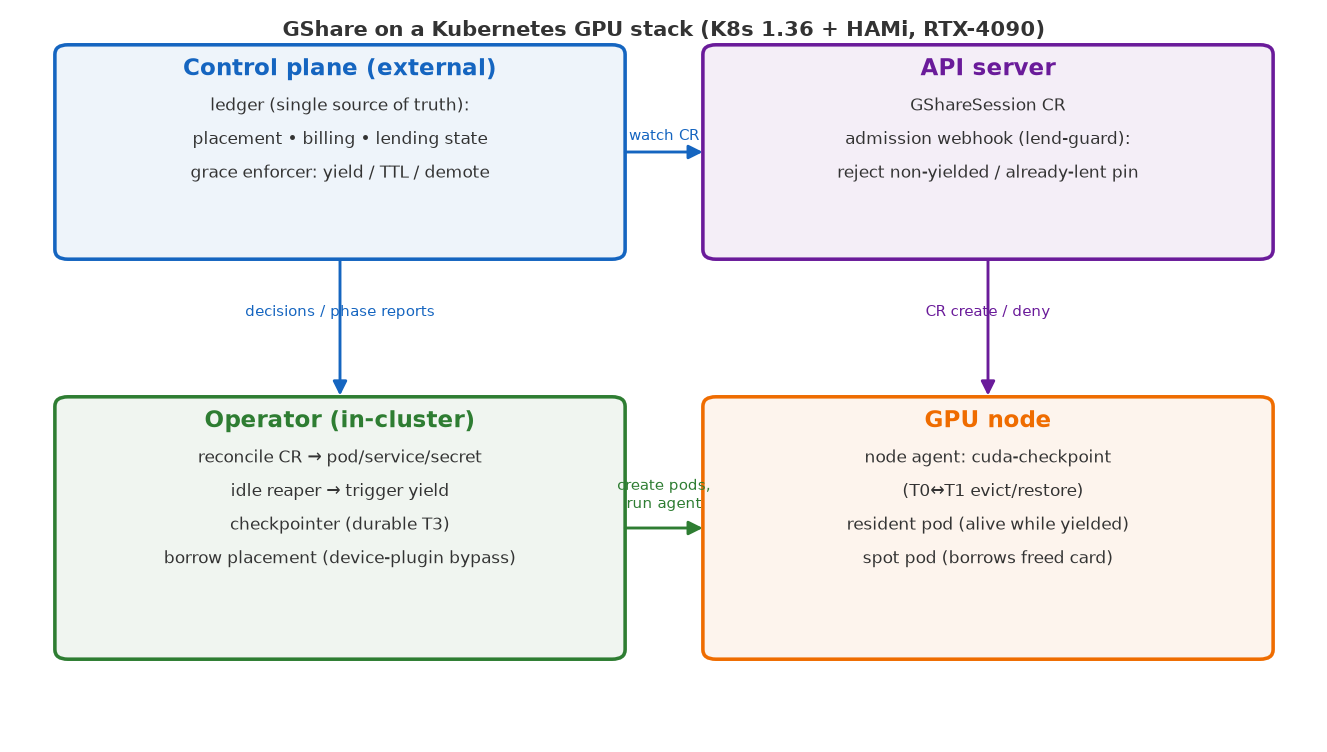
\includegraphics[width=0.96\linewidth]{arch.png}
\caption{GShare on a Kubernetes GPU stack. The control-plane ledger is the single source of truth for
placement, billing, and lending; the operator and node agent perform physical yield/borrow/reclaim; the
admission webhook enforces the lending invariant at the API server.}
\label{fig:arch}
\end{figure}

\subsection{The organizing principle: GPU occupancy as a memory hierarchy}
\label{sec:hierarchy}
The core of GShare is a single principle: \emph{GPU occupancy is not bound to the pod lifecycle; it is a
position in a memory hierarchy}. A session's VRAM working set can move losslessly between media of
differing cost and capacity, each a tier (Figure~\ref{fig:hierarchy}):

\begin{itemize}
\item \textbf{T0 --- VRAM (executing).} The session computes; it occupies the physical card.
\item \textbf{T1 --- host RAM (in-place yield).} \texttt{cuda-checkpoint} evicts the VRAM working set into
the still-running process's host memory \emph{without killing the pod}. The physical card is freed; the
process, its CUDA restore thread, the network namespace, and the pod stay alive. Restore toggles the
working set back into the same process: bit-exact, no CRI involvement. Cost: $\sim$0.2\,s/GB
(Section~\ref{sec:eval}); capacity: bounded by host RAM.
\item \textbf{T2 --- disk/NVMe (swap spill).} Under host-RAM pressure, the evicted T1 buffer is paged to
disk. We measure that the buffer is ordinary \emph{anonymous, non-pinned} memory of the suspended process,
so the operating system's swap mechanism pages it to disk by demand and faults it back on restore---no
explicit spill code, and the pod stays alive (the CRI wall is still avoided). Cost: disk-bandwidth bound
(slow); capacity: disk. T2 turns the host-RAM concurrency bound into a \emph{T1 capacity}, with T2 backing
it at lower speed.
\item \textbf{T3 --- cold/durable.} An application or container checkpoint to disk that survives node
failure. Resume is a cold restart. This is the safety net when host RAM and swap cannot hold the state, the
resume reservation expires, or the node is lost.
\end{itemize}

\begin{figure}[t]\centering
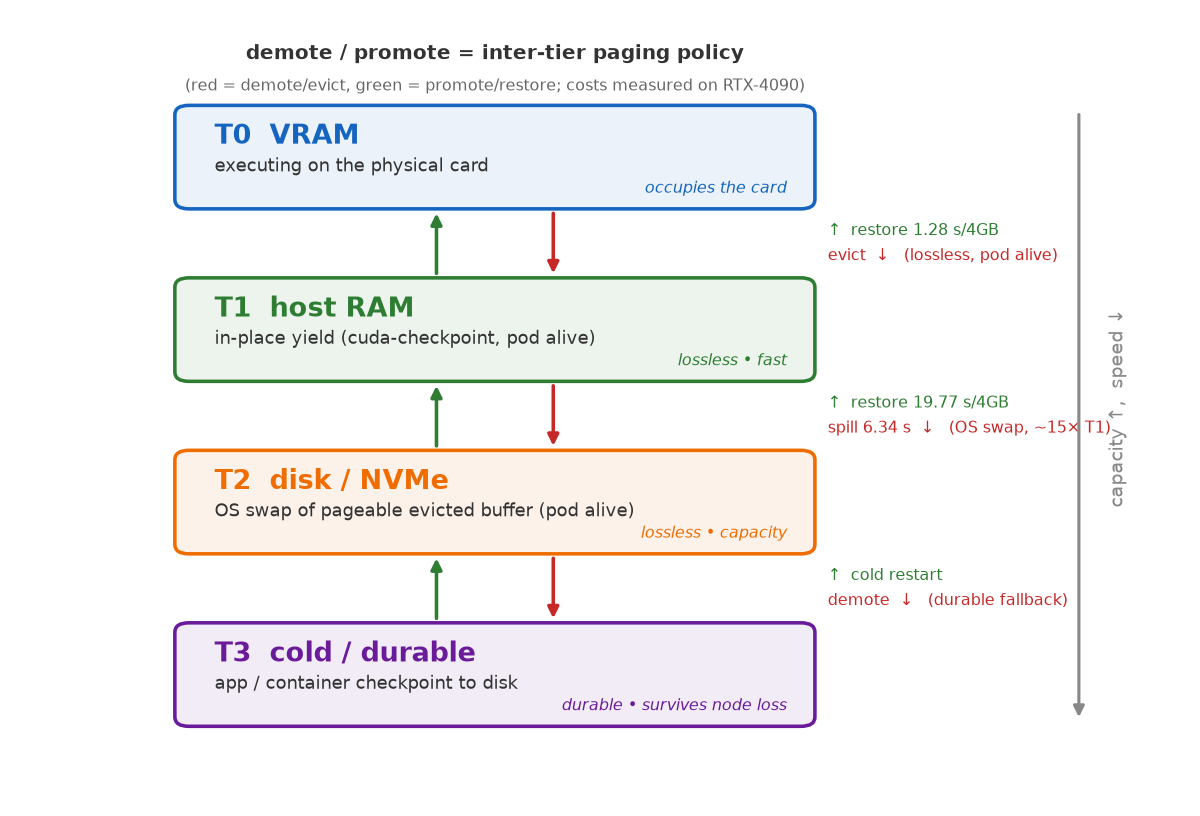
\includegraphics[width=0.8\linewidth]{hierarchy.png}
\caption{GShare models GPU occupancy as a \texttt{cache}$\leftrightarrow$\texttt{RAM}$\leftrightarrow$%
\texttt{swap} memory hierarchy. Demotion/promotion between tiers is the inter-tier paging policy
(Section~\ref{sec:policy}); transition costs are measured on RTX-4090 (Section~\ref{sec:eval}).}
\label{fig:hierarchy}
\end{figure}

This abstraction is what makes the Kubernetes CRI restore wall (Section~\ref{sec:c2}) irrelevant: because
T0$\rightarrow$T1 keeps the pod alive, no restore-as-pod is ever required, and the netns whose lifetime the
kubelet owns is never destroyed. It also distinguishes GShare from single-job memory swapping
(Section~\ref{sec:related}): the object that moves through the hierarchy is the whole occupancy state of a
yielded session, relocated across multi-tenant boundaries, not the tensors of one oversubscribed job.

\subsection{In-place GPU yield and preemptible lending}
When a resident session yields (T0$\rightarrow$T1), GShare marks its card reclaimable and admits a
preemptible \emph{spot} session onto the freed card. We use \emph{resident} for the yielding session and
\emph{spot} for the preemptible borrower. Two invariants make lending safe. First, a card carries at most
one spot session at a time; concurrent borrow claims are serialized through an atomic ledger claim and
rejected at the API server by an admission webhook (Section~\ref{sec:impl}). Second, the resident does not
\emph{own} the card while yielded---it holds a time-limited \emph{resume reservation} and its pinned host
state, nothing more---so the scheduler is free to reclaim the card when the reservation lapses. When the
resident returns within its reservation, GShare preempts the spot session and restores the resident
losslessly (T1$\rightarrow$T0); the spot session is a best-effort tenant that expects preemption.

\subsection{Preemption as an economic/paging control problem}
\label{sec:policy}
Because a yielded session occupies a hierarchy tier rather than the card, preemption becomes a control
problem over tier placement rather than a binary stop/restart. GShare expresses it as two policies. (i) A
\emph{time-limited resume reservation} (TTL) bounds how long a yielded resident may hold its lossless tier
before the card and its priority are returned; this is the fairness knob that prevents indefinite holding.
(ii) \emph{Demotion/promotion} move a session between tiers: a hot session likely to resume soon is kept in
T1; under host-RAM pressure it is demoted to T2; on TTL expiry, node loss, or when a durable checkpoint
makes cold restart cheap, it is demoted to T3. Pricing multipliers (e.g., spot discounts) are a deployment
knob, not part of the contribution.

\paragraph{Tier-selection rule.}
T2 is lossless but slow, so it is not uniformly preferable to T3. GShare selects the tier that minimizes
\emph{(resume latency $+$ expected progress redo)} subject to host-RAM and durability constraints. T1 is
chosen whenever the state fits host RAM (fast, lossless). Under host-RAM pressure, T2 beats T3 only when the
progress redo avoided by losslessness exceeds T2's extra swap-in latency---i.e., for large stateful
workloads without a cheap application checkpoint; otherwise T3 wins (durable, faster cold resume). We
ground this boundary in measured constants in Section~\ref{sec:eval}.

\subsection{Durable fallback}
The lossless tiers (T1, T2) are volatile and node-local: a node reboot or loss discards host RAM and swap.
GShare therefore falls back to T3 to preserve progress durably. A non-lent card demotes by toggling its
VRAM back and taking a fresh checkpoint on \texttt{SIGTERM} (enforced by GShare), preserving the
\emph{latest} progress; a lent card relies on the borrower's application-level periodic checkpoints. Thus
lossless yield is a fast-reclaim optimization layered on a durable safety net, not a replacement for it.

%==================================================================
\section{Implementation}
\label{sec:impl}

GShare runs on Kubernetes~1.36 with the HAMi device plugin on RTX-4090 nodes; the control plane is an
external service (FastAPI backend $+$ PostgreSQL). The implementation separates a control plane that
\emph{decides} from an execution plane that \emph{acts}.

\paragraph{Session resource and state machine.}
A session is a \texttt{GShareSession} custom resource (CR). Its spec carries the allocation mode
(fractional/exclusive), the pause mode (\texttt{cold} or \texttt{yield}), a \texttt{preemptible} flag (spot
sessions), and, for a borrower, the \texttt{borrowedGpuUuid} of the lent card; its status carries the
occupancy phase, the bound GPU UUID, the lending state, and the checkpoint reference. The resident's
occupancy evolves through the state machine of Figure~\ref{fig:statemachine}:
$\textsf{active}\rightarrow\textsf{yielded}\rightarrow\textsf{lent}\rightarrow\textsf{active}$ on the fast
lossless path, with a $\textsf{yielded}/\textsf{lent}\rightarrow\textsf{demoted}$ branch to the durable
tier on TTL expiry, host-RAM pressure, or node loss. The reclaiming step (preempt the spot, restore the
resident) is a transient transition, not a resting state; a spot session is a best-effort tenant that
expects preemption at any time within the resident's resume reservation.

\begin{figure}[t]\centering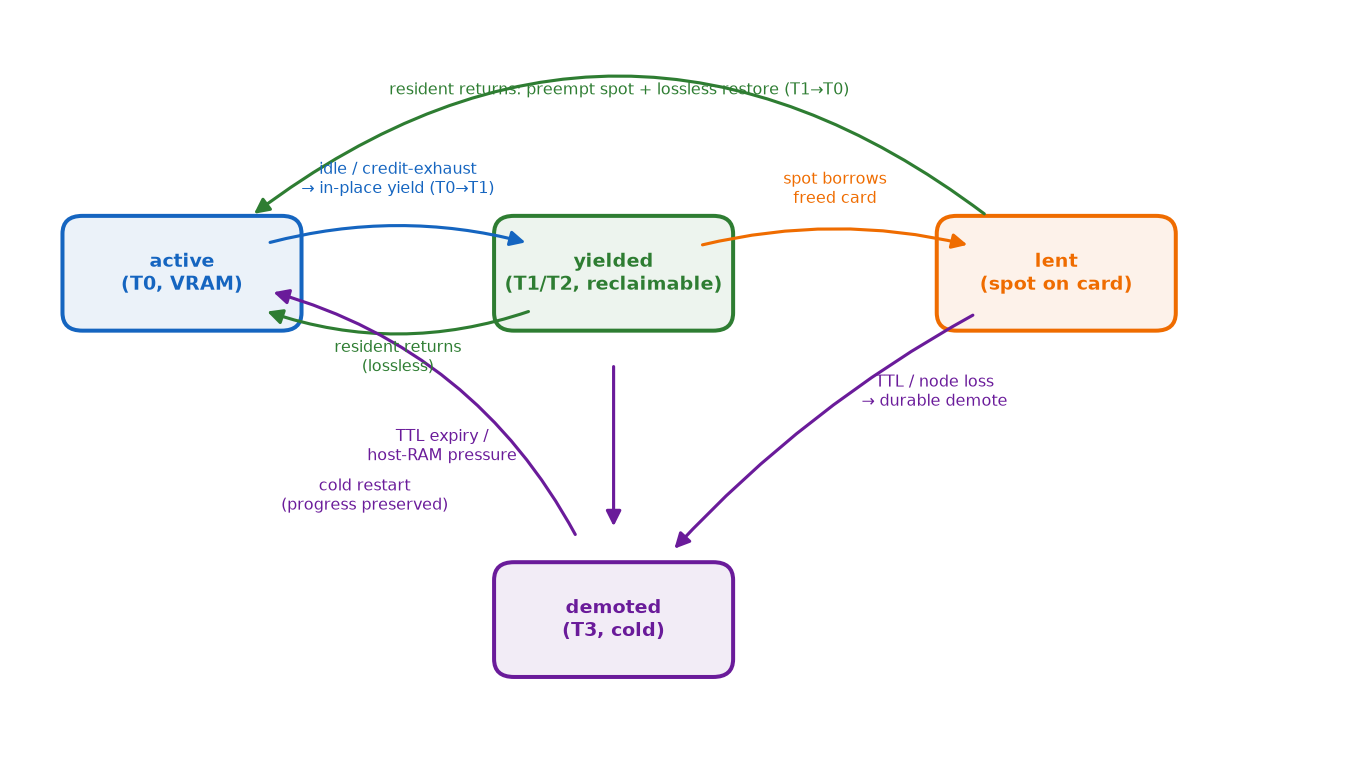
\includegraphics[width=0.9\linewidth]{statemachine.png}
\caption{Resident session occupancy state machine. Green = lossless restore (T1/T2$\rightarrow$T0); purple
= durable demotion (T3) on TTL expiry, host-RAM pressure, or node loss, with cold restart preserving
progress. A card holds at most one spot session at a time.}\label{fig:statemachine}\end{figure}

\paragraph{Control plane (single source of truth).}
A PostgreSQL ledger is the single source of truth for placement, billing, and lending state. A scheduler
computes occupancy-aware placement (a two-dimensional best-fit over VRAM and cores) and reserves both
resident and borrow slices through atomic, serialized claims, so a card is never double-lent. A billing
engine charges residents for \emph{active} card-time and stops the charge while a session is yielded. A
grace enforcer drives the economic policy: on credit exhaustion or idle, it triggers yield; it enforces the
resume-reservation TTL and the host-RAM-pressure demotion that selects victims by priority and age.

\paragraph{Operator and node agent.}
A Go operator reconciles a \texttt{GShareSession} custom resource into pods, services, and per-session
secrets, and reports phase transitions to the ledger (the ledger is the authority; the operator's reports
are fire-and-forget). An idle reaper detects idle GPUs and triggers in-place yield. Physical
yield/restore is performed by a node agent that runs \texttt{cuda-checkpoint} against the resident process;
a containerd-native checkpointer provides the durable (T3) path. In the deployed system the operator
launches the agent as a privileged, host-PID Kubernetes Job per operation; Section~\ref{sec:eval} shows
this Job orchestration---not the checkpoint mechanism---dominates reclaim latency, and that a long-lived
resident agent removes it.

\paragraph{Admission webhook and borrow placement.}
The lending invariant (one spot session per card) is enforced at two layers: the operator's in-process
reconcile and an API-server admission webhook that rejects, at \texttt{CREATE} time, any pod pinning a
non-yielded or already-lent card. Borrow placement bypasses the device plugin: because a yielded
resident's pod stays alive, it still holds the card's device-plugin allocation, so the scheduler would
consider the card full. GShare therefore places the spot pod by injecting the freed card by UUID
(\texttt{NVIDIA\_VISIBLE\_DEVICES}) with no \texttt{nvidia.com/gpu} request and a node pin---a deliberate
device-plugin bypass whose accounting is reconciled by the ledger. Integrating this with the standard
scheduler is left to future work. For isolation, the spot pod runs in its own PSA-restricted namespace and
is granted only the freed card by UUID; the resident's evicted state lives in the resident pod's own host
memory and is unreachable from the spot. Only the node agent is privileged (host-PID), so the trusted
surface is the agent, not the tenant pods.

\paragraph{Concurrency and failure handling.}
Lending claims are atomic at the database: a borrow acquires the card row under \texttt{SELECT~FOR
UPDATE}, checks it is \textsf{yielded} and unlent, and writes the claim in one transaction, so two
borrowers cannot win the same card; the admission webhook is the second, API-server-level guard. The
system degrades safely: if a checkpoint (yield) fails, the operator falls back to a cold pause rather than
risk the card; if a reclaim's lossless restore fails or the resume reservation has expired, the session is
demoted to the durable T3 tier (cold restart with the latest checkpoint) rather than lost; if the operator
crashes, it rebuilds state by reconciling the CRs against the ledger (the single source of truth), and
fire-and-forget phase reports that were missed are recomputed from observed pod state. Node loss discards
the volatile T1/T2 tiers, which is exactly why a non-lent card takes a fresh \texttt{SIGTERM} checkpoint on
demotion and a lent card relies on the borrower's periodic checkpoints (Section~\ref{sec:design}).

%==================================================================
\section{Evaluation}
\label{sec:eval}

We ask whether GShare's claimed capability is (i) characterized at the mechanism level, (ii)
functionally correct, (iii) advantageous against alternative design points, and (iv) able to scale. The
evaluation spans three buckets: (1) the live GShare system, (2) bare-GPU baselines, and (3) a
trace-driven simulator. Table~\ref{tab:results} maps each claim to its evidence and headline result;
the subsections that follow elaborate. All figures and the commands to reproduce them are in the artifact.

\begin{table*}[t]\centering\small
\caption{Roadmap of claims, evidence, and headline results.}
\label{tab:results}
\begin{tabular}{@{}p{0.30\linewidth}p{0.20\linewidth}p{0.44\linewidth}@{}}
\toprule
Claim & Evidence & Headline result \\
\midrule
Lossless yield mechanism is cheap & \S\ref{sec:eval} M1, Fig.~\ref{fig:mechgroup} & 6\,GB restore 1.74\,s, restore $3\times$ faster than evict, \textbf{0 progress lost} \\
Full lifecycle works live & Fig.~\ref{fig:fv1} & yield$\rightarrow$borrow$\rightarrow$reclaim verified on hardware, lossless \\
Space-sharing cannot give a full card & Fig.~\ref{fig:e1}; real MPS & each co-tenant $\sim\frac{1}{2}$ (MPS 27.3/27.5 vs solo 54.7\,TF) \\
Lossless resume beats alternatives & Fig.~\ref{fig:e1b} & GShare 1.74\,s $<$ cold-STOP 4.75\,s $<$ app-ckpt $\sim$9\,s \\
Losslessness matters for stateful jobs & Fig.~\ref{fig:p0group} & cold-STOP redoes minutes (large model); GShare \textbf{0 redo} \\
Real multi-tenant recovers idle cards & Fig.~\ref{fig:mt} & keep-idle 0 $\rightarrow$ GShare 109\,TFLOPS, lossless reclaim \\
Cluster benefit (cross-validated sim) & Fig.~\ref{fig:simgroup} & occupancy $2.4\times$ at low duty; simulator 19/19 validated \\
Real-trace grounding (honest bound) & Fig.~\ref{fig:tracegroup} & 58.8\% of GPU-time $<$25\% util; reclaim bound 0--223 GPU-h/24\,h \\
Reclaim is orchestration-bound & Fig.~\ref{fig:reclaim} & Job 8.2\,s vs.\ resident agent 1.28\,s ($6.4\times$) \\
host-RAM bound is a T1 capacity; T2 is real & Fig.~\ref{fig:hostram} & T2 spill 6.34\,s $+$ restore 19.77\,s, lossless \\
Control-plane overhead is negligible & \S\ref{sec:eval} O1 & scheduling P99 0.04\,ms, ledger P99 1.2\,ms \\
\bottomrule
\end{tabular}
\end{table*}

\subsection{Experimental setup}
The testbed is a two-node GPU cluster (gpu2-1, gpu2-2; each RTX-4090, 24\,GB, 64\,GiB host RAM, driver
595, CUDA 13.2) running Kubernetes~1.36 with the HAMi device plugin (10 slices/node); the control plane
runs externally (FastAPI $+$ PostgreSQL). The microbenchmark workload is a single cuBLAS SGEMM loop that
independently controls VRAM footprint and compute and reports measured throughput; the stateful workload
is real training (Section~\ref{sec:eval-stateful}).

\paragraph{Artifact and reproducibility.}
A reproducibility artifact accompanies the paper [REPO/DOI]: it contains the measurement scripts, raw data
(CSV/logs), and figure-generation sources for every figure and number reported here, together with a
per-figure index of the exact command that regenerates it. The simulator is seed-fixed and deterministic;
its cross-validation harness (V1--V3) is included and asserts the cost-model fit and aggregation
correctness on each run. The Alibaba PAI 2020 trace used in Sections~\ref{sec:eval} is publicly released by
its authors~\cite{mlaas}; our parsing scripts are in the artifact. Live-cluster experiments require a
GPU Kubernetes testbed and are documented with the manifests and procedures used.

\subsection{Mechanism: cost of in-place yield (T0$\leftrightarrow$T1)}
We characterize the lossless-yield mechanism over VRAM footprint (Figure~\ref{fig:m1}, $N{=}5$, measured
on the node via the driver API). Both eviction and restore are linear in footprint; restore is $\sim3\times$
faster than eviction ($\sim$3.5 vs $\sim$1.2\,GB/s). Lossless resume for a 6\,GB working set is 1.74\,s---%
faster than the same node's cold-start floor---and, decisively, preserves state exactly (zero progress
lost). One yield cycle costs $W^{*}{=}\text{evict}{+}\text{restore}$ of non-productive GPU time, so a
borrow window $W$ yields net recovery only when $W{>}W^{*}$; the recovered spot GPU-time is
$\max(0, W{-}W^{*})$ and the break-even window grows with model size (Figure~\ref{fig:m5}). During the
window the borrower holds the full card and recovers 54\,TFLOPS (fp32), versus zero under keep-idle.

\begin{figure}[t]\centering
\begin{subfigure}{0.42\linewidth}\centering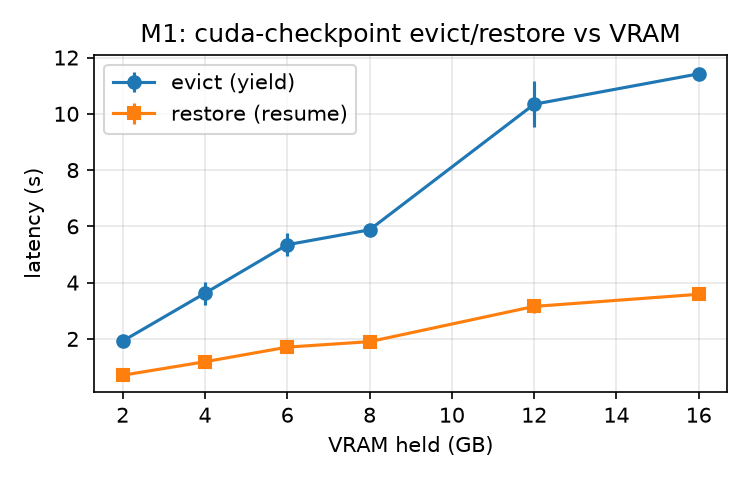
\includegraphics[width=\linewidth]{m1.png}
\caption{Evict/restore vs.\ footprint.}\label{fig:m1}\end{subfigure}\hfill
\begin{subfigure}{0.56\linewidth}\centering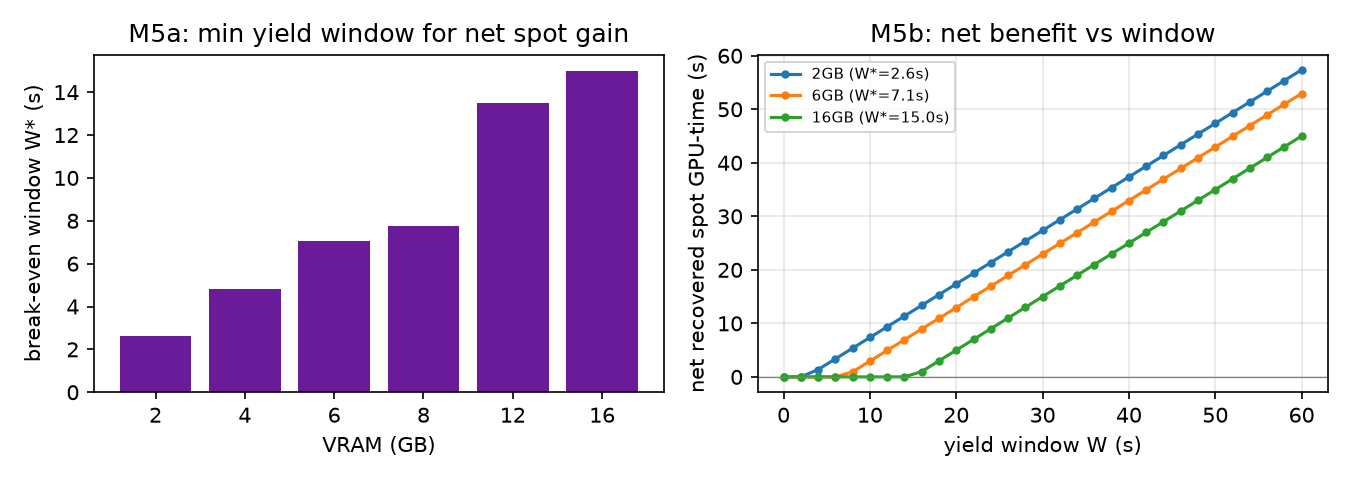
\includegraphics[width=\linewidth]{m5.png}
\caption{Break-even.}\label{fig:m5}\end{subfigure}
\caption{Mechanism cost of in-place yield (RTX-4090, $N{=}5$). (a) evict/restore latency is linear in VRAM
footprint, restore $\sim3\times$ faster than evict. (b) round-trip overhead $W^{*}{=}$evict$+$restore and
net recovered spot GPU-time $\max(0,W{-}W^{*})$ vs.\ window $W$.}\label{fig:mechgroup}\end{figure}

\subsection{Functional validation}
We confirm the full lifecycle live on gpu2-1 (Figure~\ref{fig:fv1}): resident active $\rightarrow$ yield
(VRAM evicted, pod alive) $\rightarrow$ spot borrows the full card $\rightarrow$ reclaim (lossless restore)
$\rightarrow$ resident active, continuing from the exact step. Controlled tests further validate
occupancy-aware placement, the CRI-restore negative result (Section~\ref{sec:c2}, reproduced live), the
lending invariant enforced at both the operator and the admission webhook, host-RAM-pressure demotion
(lowest-priority/oldest first), and the durable graceful-demotion fallback.

\begin{figure}[t]\centering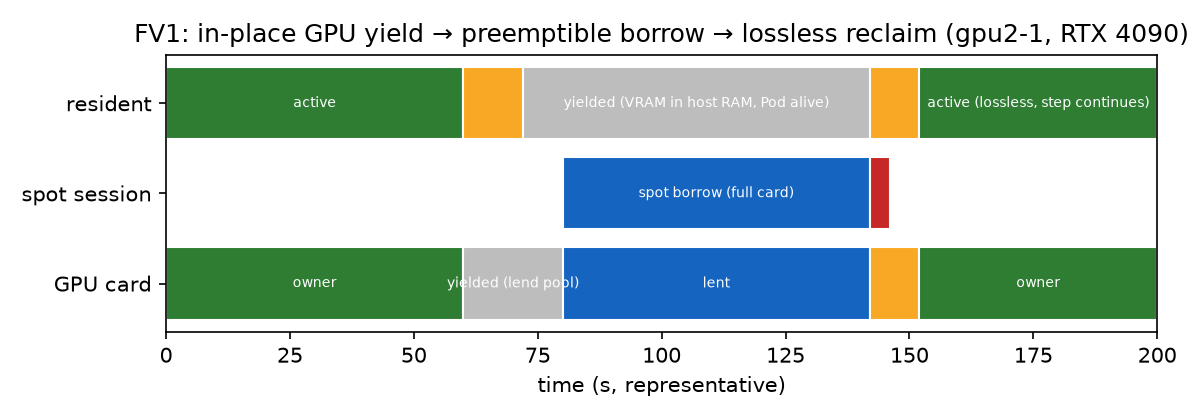
\includegraphics[width=0.92\linewidth]{fv1.png}
\caption{Live yield$\rightarrow$borrow$\rightarrow$reclaim lifecycle (RTX-4090, operator logs). The spot
holds the full card during the yield window and is preempted on the resident's lossless return.}
\label{fig:fv1}\end{figure}

\subsection{Five-condition comparison against alternative design points}
On one identical scenario (6\,GB SGEMM; resident burst$\rightarrow$idle$\rightarrow$burst with a spot
targeting the idle window) we compare GShare to four alternative points (Figure~\ref{fig:e1}). Read along
three axes. (1) \emph{Reclaim?}---only keep-idle recovers nothing (spot is scheduling-blocked).
(2) \emph{How?}---\texttt{concurrent-share} (space-sharing, the family of MPS/HAMi/Orion) co-locates and
gives each job one-half (each $\sim$26.5\,TF, $2\times$ slowdown), and varying the core split 50:50/70:30/90:10
still converges to one-half, showing space partitioning cannot grant full throughput under SM saturation;
cold-STOP, app-checkpoint, and GShare instead serialize at full card (54\,TF each). We confirm the
one-half ceiling on \emph{real NVIDIA MPS}: solo 54.69\,TF vs.\ a 2-way co-location of 27.27/27.49\,TF---%
the family's fundamental cost, not a HAMi artifact. (3) \emph{Resident resume cost} (the differentiator
among the serial-reclaim conditions, Figure~\ref{fig:e1b}): GShare 1.74\,s (lossless, pod alive) $<$
cold-STOP 4.75\,s (cold restart, state lost) $<$ app-checkpoint $\sim$9\,s (cold restart $+$ disk-checkpoint
load, durable). App-checkpoint trades latency for durability; GShare trades volatility for speed---they
occupy opposite ends of the same axis. Figure~\ref{fig:e2} decomposes card-time: only keep-idle wastes the
idle window; GShare wastes none beyond the lossless round-trip. GShare is thus \emph{orthogonal} to
space-sharing: when the resident is idle there is no co-runner to share with, so the card is reclaimed
whole and losslessly.

\begin{figure}[t]\centering
\begin{subfigure}{0.74\linewidth}\centering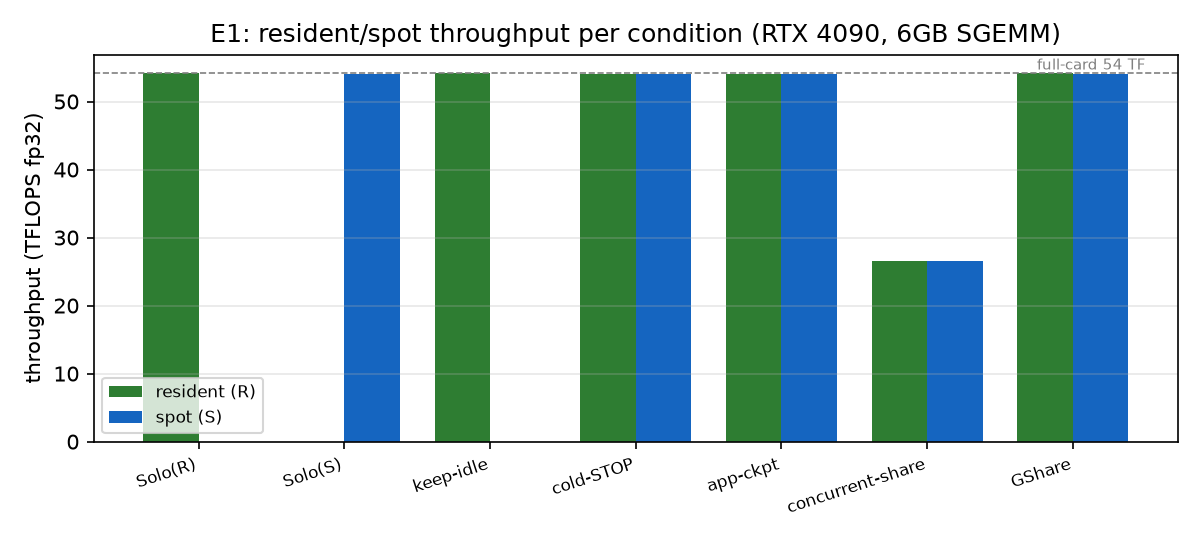
\includegraphics[width=\linewidth]{e1.png}
\caption{Per-condition resident/spot throughput.}\label{fig:e1}\end{subfigure}

\medskip
\begin{subfigure}{0.49\linewidth}\centering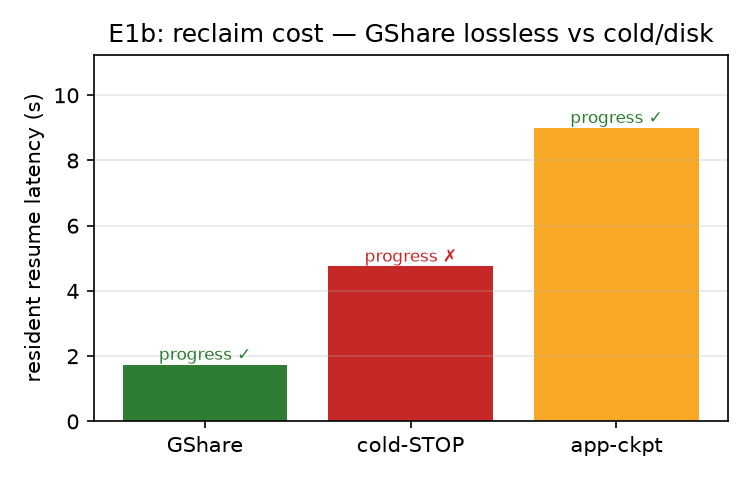
\includegraphics[width=\linewidth]{e1b.png}
\caption{Resident resume-cost spectrum.}\label{fig:e1b}\end{subfigure}\hfill
\begin{subfigure}{0.49\linewidth}\centering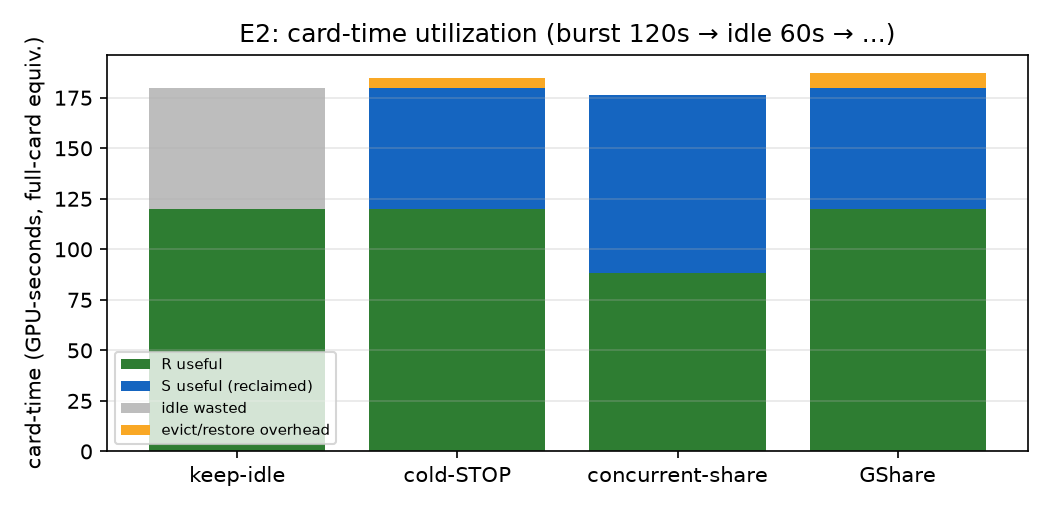
\includegraphics[width=\linewidth]{e2.png}
\caption{Card-time decomposition.}\label{fig:e2}\end{subfigure}
\caption{Five-condition comparison (6\,GB SGEMM). (a) keep-idle: spot blocked (0); concurrent-share: each
one-half (26.5\,TF); cold-STOP/app-ckpt/GShare: serial full card (54\,TF each). (b) resident resume cost
among serial-reclaim conditions: GShare (lossless) 1.74\,s $<$ cold-STOP (state lost) 4.75\,s $<$
app-checkpoint (durable) $\sim$9\,s. (c) card-time for burst$\rightarrow$idle$\rightarrow$burst: only
keep-idle wastes the idle window; GShare adds only the lossless round-trip.}\label{fig:e1group}\end{figure}

\subsection{Stateful workloads: the value of losslessness}
\label{sec:eval-stateful}
The SGEMM comparison understates cold-STOP's cost because it is stateless (no progress to redo). With real
training (Figure~\ref{fig:p0}), a burst preempted mid-interval forces cold-STOP to reload the last disk
checkpoint and redo the lost steps, whereas GShare's in-place yield resumes at the exact step with zero
redo. For large models the gap is minutes, not seconds (Figure~\ref{fig:p0scale}): a ViT-L+Adam checkpoint
is 3.48\,GB and takes $\sim$27\,s to write, forcing minute-scale checkpoint intervals, so a random
preemption redoes minutes of work plus a measured 12.87\,s cold start; GShare's lossless restore
(3.58\,s, disk-free) is flat in model size. The lossless advantage therefore grows with model size.

\begin{figure}[t]\centering
\begin{subfigure}{0.49\linewidth}\centering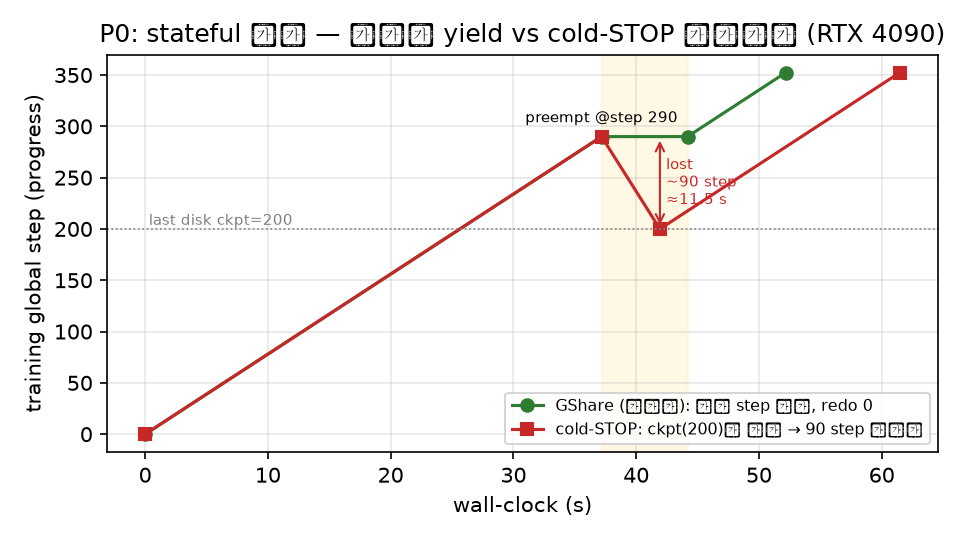
\includegraphics[width=\linewidth]{p0_train.png}
\caption{Progress vs.\ wall-clock.}\label{fig:p0}\end{subfigure}\hfill
\begin{subfigure}{0.49\linewidth}\centering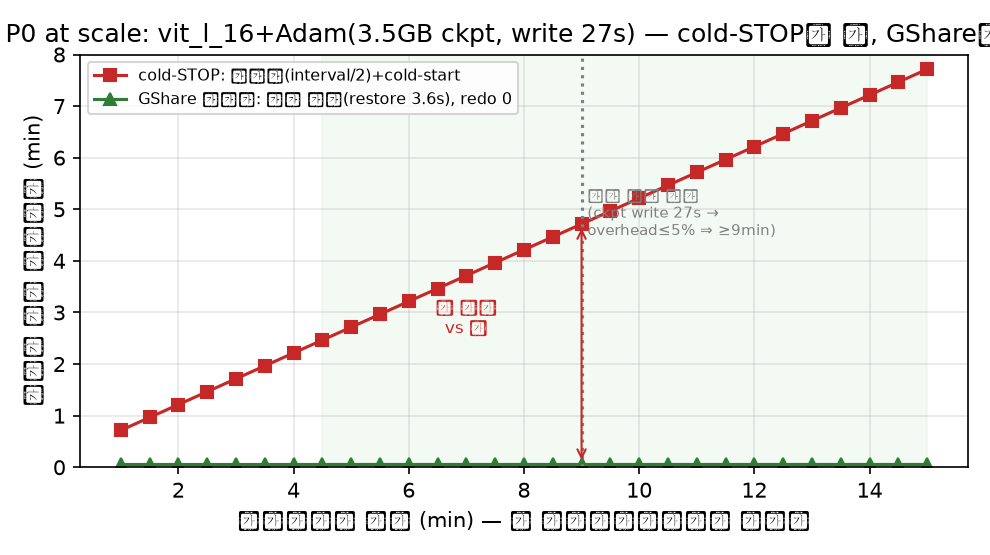
\includegraphics[width=\linewidth]{p0_scale.png}
\caption{Expected loss vs.\ checkpoint interval.}\label{fig:p0scale}\end{subfigure}
\caption{Stateful training. (a) cold-STOP rolls back to the last disk checkpoint and redoes steps; GShare
resumes losslessly (zero redo). (b) for large models (ViT-L+Adam) the per-preemption loss is minutes
while GShare stays flat at the lossless restore.}\label{fig:p0group}\end{figure}

\subsection{Real two-node multi-tenant yield/borrow/reclaim}
We run the capability live across both nodes (Figure~\ref{fig:mt}): two resident sessions (one per node,
4\,GB each) idle-hold their cards (keep-idle: zero useful work), GShare yields both in place (VRAM
$4492{\to}1$\,MiB), lends each freed card to a spot session via device-plugin-bypass placement, and reclaims
both losslessly. Result: keep-idle recovers 0 useful TFLOPS from the two idle cards, whereas GShare recovers
109.1\,TFLOPS aggregate ($2{\times}54.5$, full card, 100\% utilization) and restores the residents losslessly
(state \texttt{running}, VRAM restored, 1.26/1.67\,s). This realizes the keep-idle-vs-GShare and full-card
claims on real multi-tenant hardware rather than in simulation.

\begin{figure}[t]\centering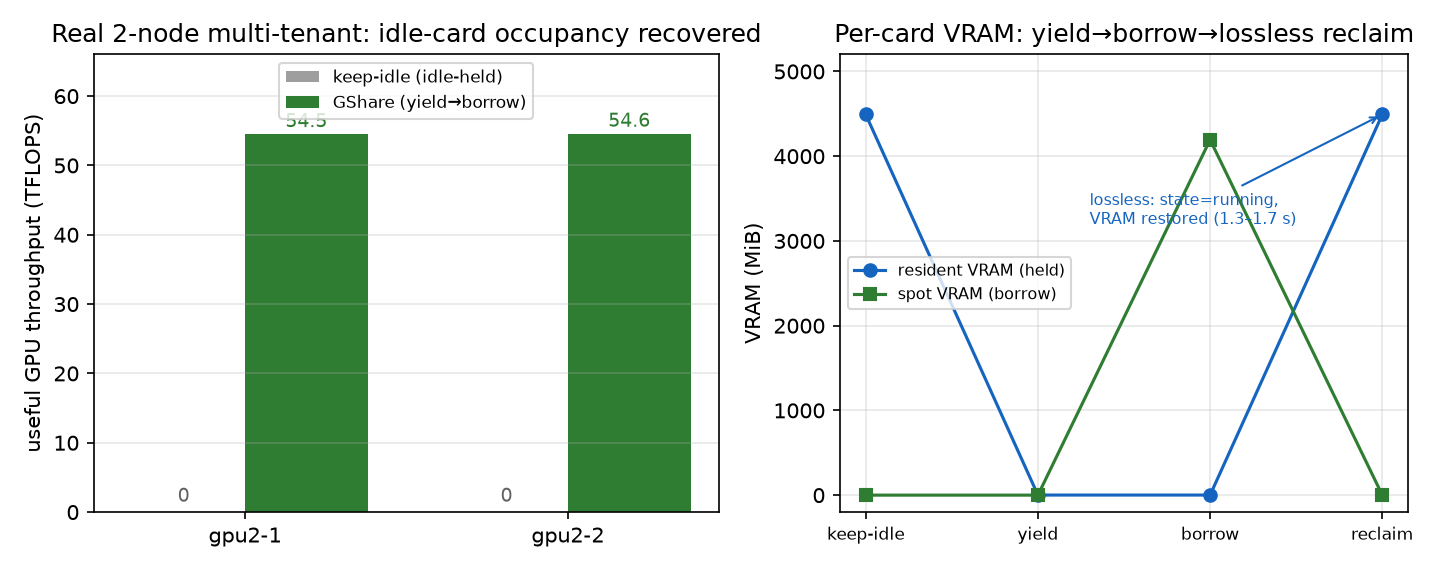
\includegraphics[width=0.92\linewidth]{mt_occupancy.png}
\caption{Real two-node multi-tenant. (left) useful throughput recovered from idle cards: keep-idle 0 vs.\
GShare $\sim$54.5\,TF each. (right) per-card VRAM across yield$\rightarrow$borrow$\rightarrow$lossless
reclaim.}\label{fig:mt}\end{figure}

\subsection{Cluster-scale simulation and its validation}
A trace-driven discrete-event simulator parameterized by the real system constants and the M1 cost model
projects cluster effects (16 cards, 24\,h). Occupancy recovery concentrates at low resident duty cycle
(Figure~\ref{fig:s1}; $2.4\times$ at load 0.1) and vanishes at high duty where there is no idle to reclaim.
At equal occupancy, GShare's resident resume cost is $2.3$--$3.0\times$ lower than cold-preemption
(Figure~\ref{fig:s2}), and this advantage grows with cold-start cost up to $8.7\times$
(Figure~\ref{fig:s3}); we anchor cold-start on the measured 12.87\,s training value, the most conservative
choice. Treating preemption economically (Figure~\ref{fig:s4}), keep-idle bills idle-but-recoverable
GPU-time (173.6 GPU-h wasted at load 0.1) for which no work is done, while GShare converts it to useful
spot work and the resume-reservation TTL trades lossless-resume share against fair card return.

\paragraph{Cross-validation.} We establish the simulator's credibility with three independent checks
(19/19 pass): (V1) its cost functions \emph{are} the least-squares fit to the M1 data ($R^2{>}0.95$), with
cold-start anchored on the measured value; (V2) on a deterministic single-card scenario every emitted
aggregate equals an independent closed-form hand-computation to floating-point precision; (V3) a real E1
cold-preemption cycle, reconstructed as a single-card scenario, is reproduced with 0.00\% error. The
S-series claims are thus a validated deterministic composition of measured primitives, not an ungrounded
model. (Correcting an earlier unmeasured cold-start guess lowered the reported advantage from
$3.2$--$6.5\times$ to the conservative $2.3$--$3.0\times$.)

\begin{figure}[t]\centering
\begin{subfigure}{0.46\linewidth}\centering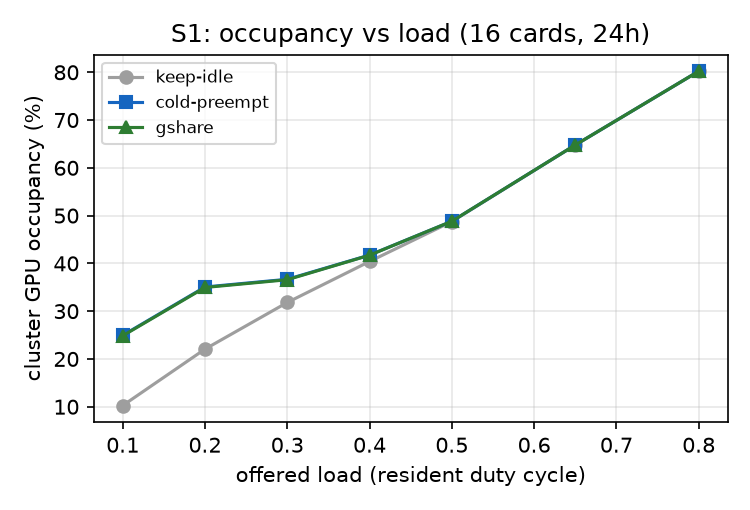
\includegraphics[width=\linewidth]{s1.png}
\caption{Occupancy vs.\ load.}\label{fig:s1}\end{subfigure}\hfill
\begin{subfigure}{0.52\linewidth}\centering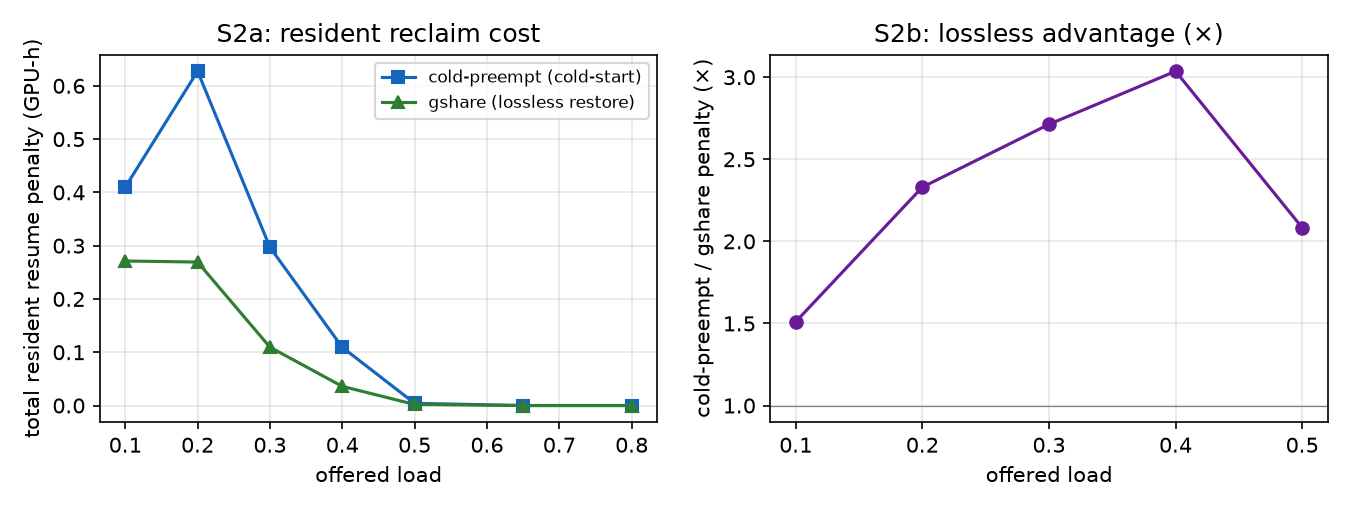
\includegraphics[width=\linewidth]{s2.png}
\caption{Resident resume cost.}\label{fig:s2}\end{subfigure}

\medskip
\begin{subfigure}{0.46\linewidth}\centering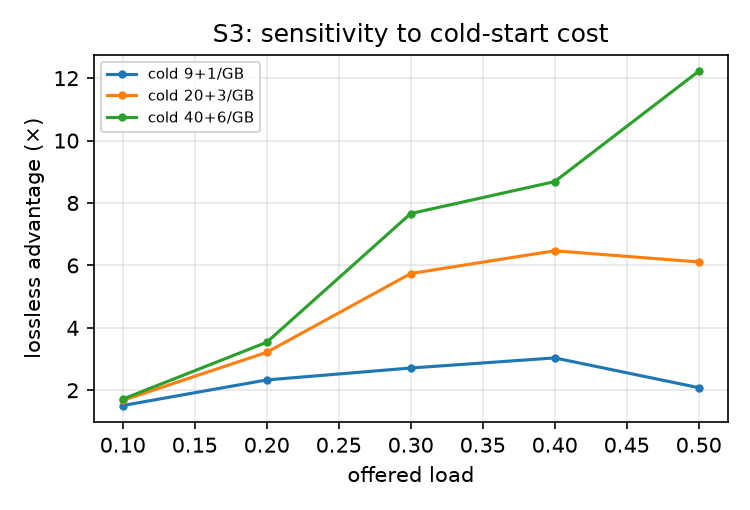
\includegraphics[width=\linewidth]{s3.png}
\caption{Cold-start sensitivity.}\label{fig:s3}\end{subfigure}\hfill
\begin{subfigure}{0.52\linewidth}\centering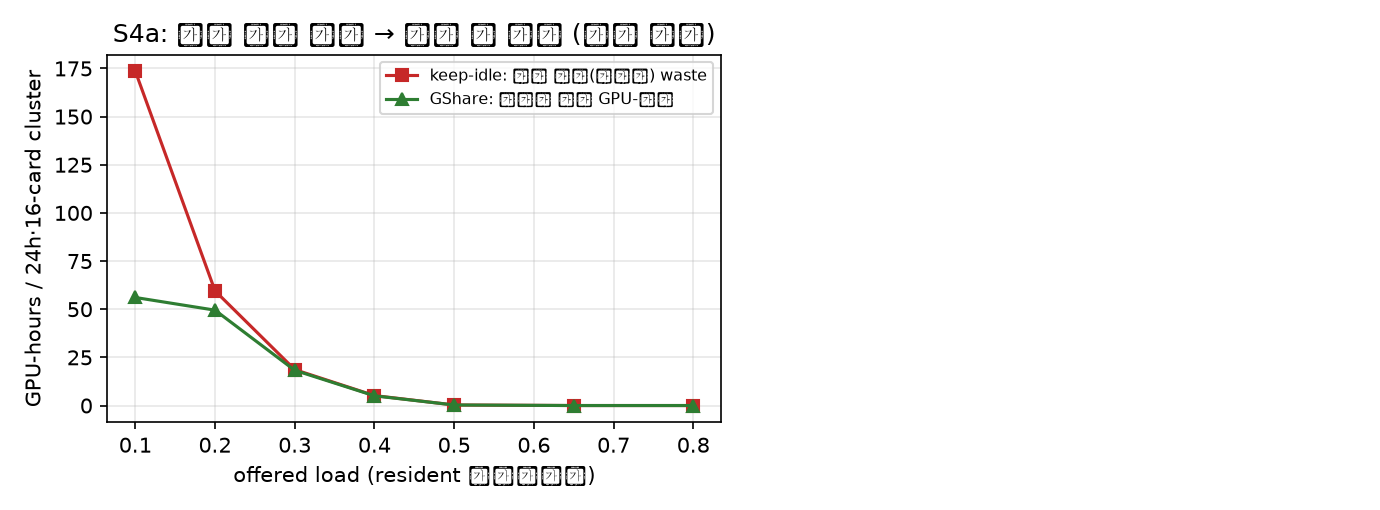
\includegraphics[width=\linewidth]{s4.png}
\caption{Reclaim economics.}\label{fig:s4}\end{subfigure}
\caption{Cluster-scale simulation (16 cards, 24\,h). (a) GShare's occupancy recovery is largest at low duty
and vanishes at high duty. (b) resident resume cost at equal occupancy: GShare (lossless) vs.\
cold-preemption. (c) sensitivity to cold-start cost; the measured anchor is the conservative lower end.
(d) reclaim economics (no pricing): keep-idle paid-but-idle waste vs.\ GShare recovered useful GPU-h, and
the resume-reservation TTL as the lossless$\leftrightarrow$durable knob.}\label{fig:simgroup}\end{figure}

\paragraph{Real-trace grounding and an honest bound.}
We ground the duty-cycle assumption in the Alibaba PAI 2020 trace~\cite{mlaas} (18.4M GPU-hours, 1814 GPU
machines). The measured per-GPU utilization distribution (Figure~\ref{fig:trace}) confirms pervasive
under-occupancy---58.8\% of GPU-time runs below 25\% utilization, 95\% below 50\%---so the cost of held-but-%
idle cards is real at scale. However, most of this is low-\emph{active} (10--50\%), the space-sharing
regime to which GShare is orthogonal; GShare's direct slice is the whole-card-idle and lossless-preemption
portion, not the 95\%. Driving the simulator with the real distribution rather than a synthetic sweep
(Figure~\ref{fig:traced}), the recovered spot GPU-time is \emph{bounded} between 0 (if all sub-full
utilization is sustained-low intensity) and 223 GPU-h/24\,h (if all is idle gaps); at the optimistic end
occupancy lifts from 28.3\% to 42.9\%. The trace cannot resolve which, because it averages utilization over
each worker's lifetime and so hides intra-session idle gaps---the very gaps GShare reclaims---so we report
the bound rather than a single figure. The bound's floor is \emph{parity, not loss}:
at every $\varphi$ GShare's occupancy is at least keep-idle's and never below it (Figure~\ref{fig:traced}),
because GShare yields only when a borrower can use the freed window and always reclaims losslessly. The
capability thus has no downside relative to the status quo---only a workload-dependent upside.

\begin{figure}[t]\centering
\begin{subfigure}{0.44\linewidth}\centering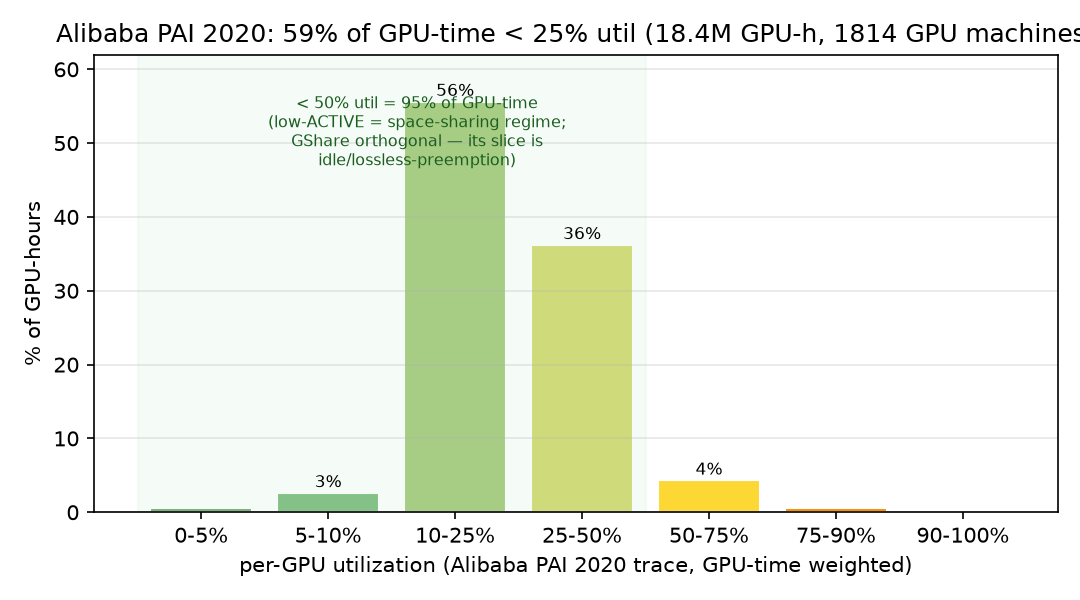
\includegraphics[width=\linewidth]{trace_impact.png}
\caption{Real util distribution.}\label{fig:trace}\end{subfigure}\hfill
\begin{subfigure}{0.54\linewidth}\centering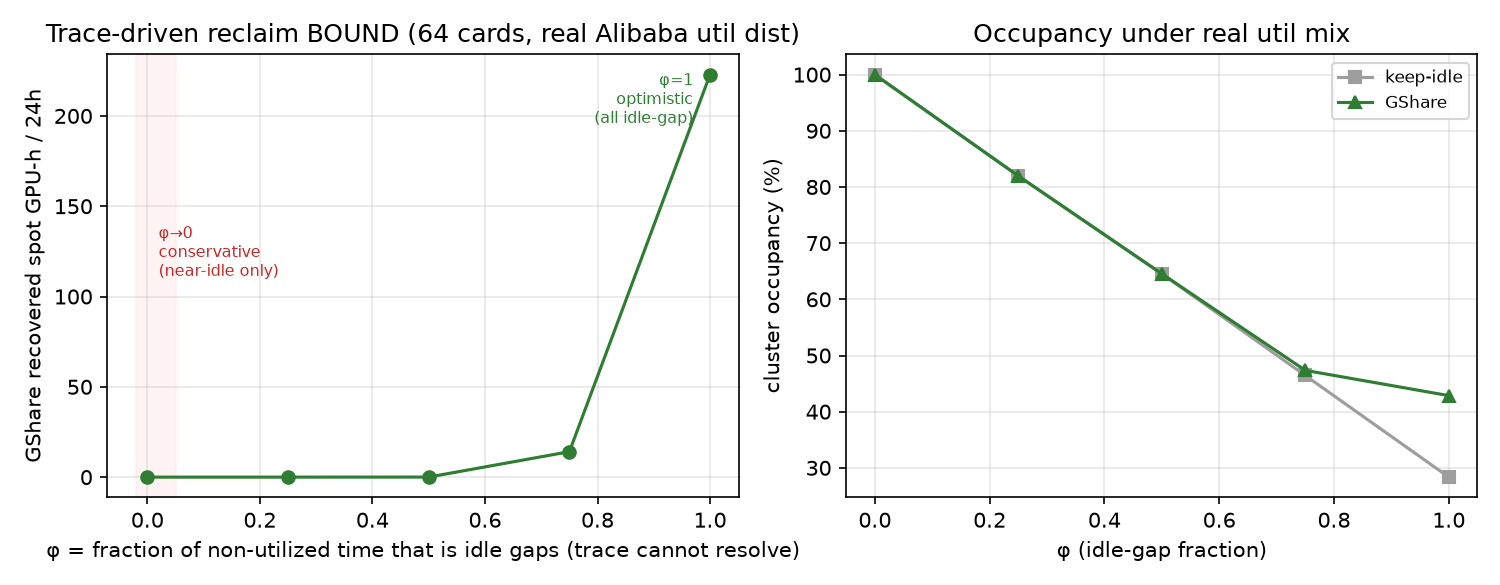
\includegraphics[width=\linewidth]{trace_driven.png}
\caption{Trace-driven reclaim bound.}\label{fig:traced}\end{subfigure}
\caption{Real-trace grounding (Alibaba PAI 2020). (a) per-GPU utilization (GPU-time weighted): 58.8\%
below 25\%, 95\% below 50\%---pervasive under-occupancy as background motivation. (b) driving the
simulator with this distribution, GShare's recovered GPU-h is bounded by the trace-unresolvable idle-gap
fraction $\varphi$; reported as an honest bound, not a single figure.}\label{fig:tracegroup}\end{figure}

\subsection{System overhead, reclaim latency, and the hierarchy in practice}
Control-plane overhead is negligible against session lifetimes: a scheduling decision is P50 0.013\,ms /
P99 0.041\,ms, a ledger transaction P50 0.80\,ms / P99 1.21\,ms, and admission-webhook P50 $<$5\,ms.

\paragraph{Reclaim latency is Job-orchestration-bound, not mechanism-bound.}
The deployed reclaim launches a privileged Job per operation and polls it; we measured both paths on the
same live 4\,GB process via a long-lived resident agent (Figure~\ref{fig:reclaim}). The Job path takes
8.2\,s (container start dominates; $+$3\,s for the operator's poll yields the observed $\sim$10\,s),
whereas a single RPC into an already-running resident agent does restore$+$unlock in 1.28\,s---a measured
$6.4\times$ reduction. The reclaim bottleneck is thus removable Job orchestration, not the cuda-checkpoint
mechanism (1.07\,s for 4\,GB, matching M1).

\begin{figure}[t]\centering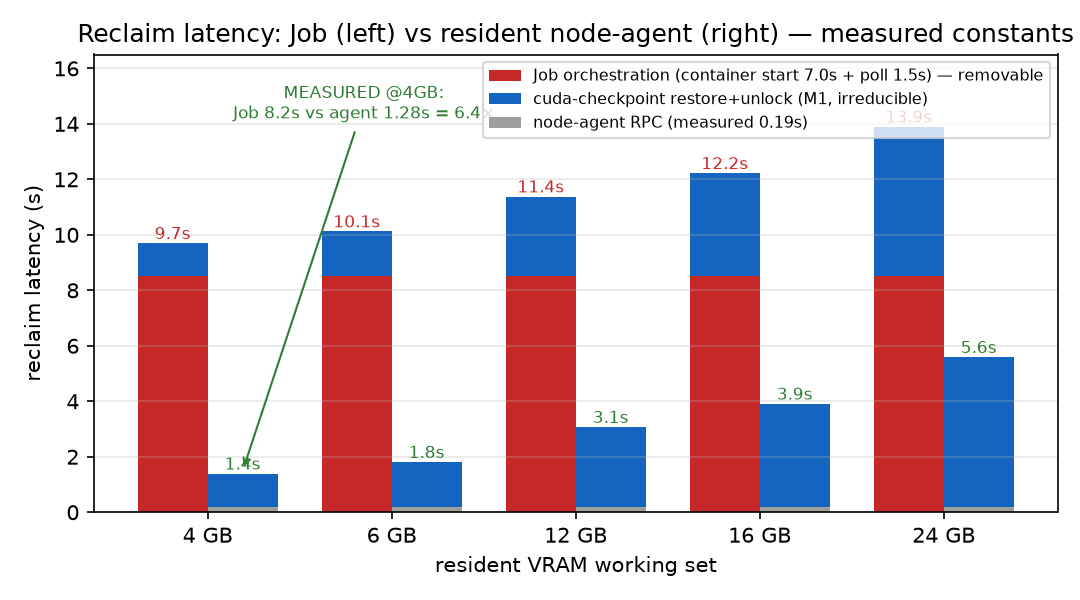
\includegraphics[width=0.92\linewidth]{reclaim_decomp.png}
\caption{Reclaim latency: per-reclaim Job (left) vs.\ resident node-agent (right), all measured. Removable
Job orchestration dominates; the resident agent leaves only the mechanism $+$ RPC.}\label{fig:reclaim}\end{figure}

\paragraph{The host-RAM bound is a T1 capacity, and T2 is real.}
The number of concurrent in-place yields per node is bounded by $\lfloor \text{host\_RAM}\times0.5/\text{VRAM}\rfloor$
(Figure~\ref{fig:hostram})---on the 64\,GiB testbed, five 6\,GB or one 24\,GB yield. But this is the
\emph{T1 capacity}, not a hard limit: we measure that the evicted buffer is anonymous, non-pinned memory
(\texttt{VmLck}{=}\texttt{VmPin}{=}0), so the OS swaps it to disk, realizing T2 losslessly with the pod
alive. End-to-end on real swap: a 4\,GB session spills to disk in 6.34\,s (freeing 4.66\,GB of host RAM)
and restores losslessly in 19.77\,s---$\sim15\times$ T1's 1.28\,s, exactly the capacity-not-speed tradeoff
of a lower tier. The concurrency bound thus becomes host-RAM$+$swap, i.e.\ hot-working-set size.
Because T2 is slow, the tier-selection rule (Section~\ref{sec:policy}) matters: from the measured swap
bandwidth ($\sim$221\,MB/s) and cold-start (12.87\,s), T2's resume exceeds cold-start beyond $\sim$3\,GB,
so T2 is chosen over the durable T3 only for large stateful workloads lacking a cheap checkpoint
(Figure~\ref{fig:tier}); otherwise T3 wins.

Keeping a yielded pod alive is not free beyond host RAM. The suspended resident still occupies a pod slot
and its reserved CPU/memory \emph{requests}, so per node the number of concurrent live-but-yielded sessions
is also bounded by the kubelet's pod-per-node limit ($\sim$110 by default) and by reserved-CPU/memory
headroom---not only by the host-RAM (T1) capacity. In practice the binding constraint is whichever is
tightest: host RAM for large working sets, pod/CPU-request density for many small sessions. T3 demotion
(which frees the pod entirely) is the release valve when pod density, rather than host RAM, is the limit.

\begin{figure}[t]\centering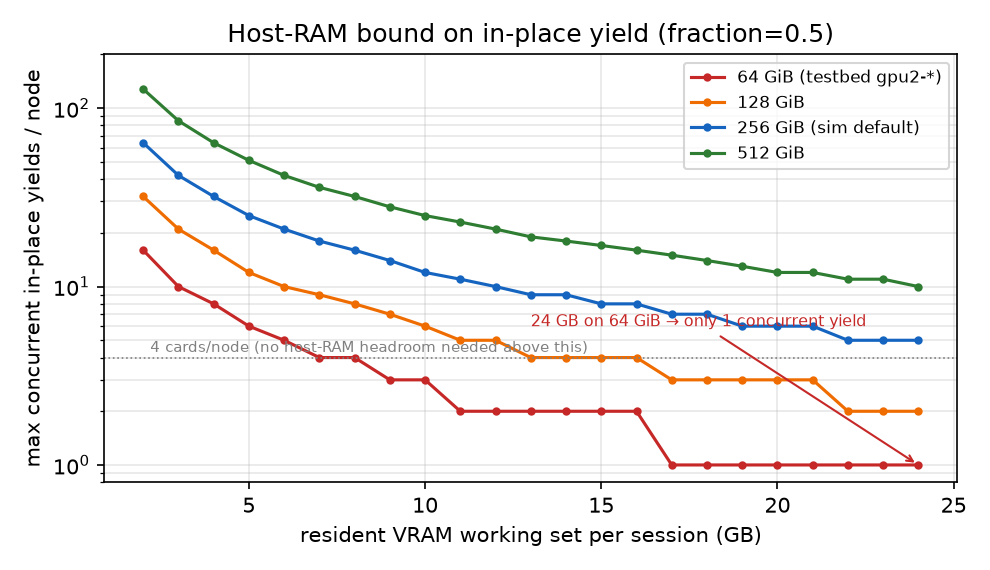
\includegraphics[width=0.7\linewidth]{hostram_bound.png}
\caption{Host-RAM bound on concurrent in-place yields per node (the T1 capacity); T2 (swap/NVMe) backs it
losslessly at lower speed.}\label{fig:hostram}\end{figure}

\begin{figure}[t]\centering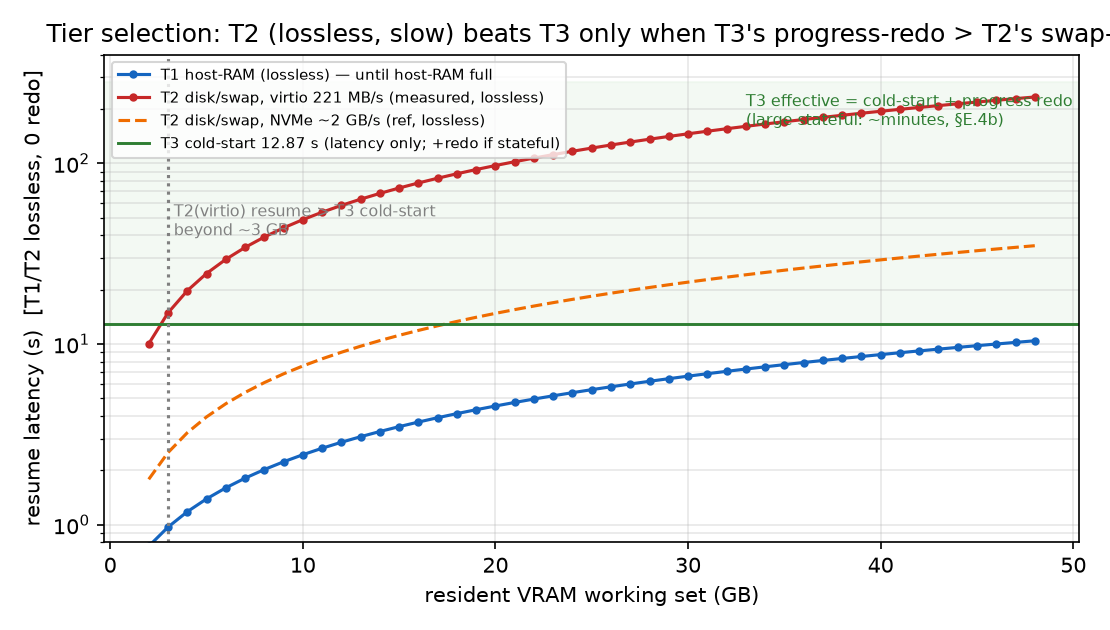
\includegraphics[width=0.82\linewidth]{tier_policy.png}
\caption{Tier-selection from measured constants: T2 (lossless, slow) beats the durable T3 only when T3's
progress redo exceeds T2's swap-in.}\label{fig:tier}\end{figure}

\subsection{Positioning}
Our measured family representatives confirm the categorical picture of Table~\ref{tab:designpoints}:
space-sharing (real MPS) cannot give a full card under SM saturation; durable preemption (app-checkpoint)
preserves progress but pays disk latency; cold-stop loses state. We attempted Orion directly but it
deadlocked on the torch/CUDA-12/RTX-4090 ABI (an honest negative), and AntMan is TensorFlow-1.x-era and not
buildable on the current stack; as argued in Section~\ref{sec:related}, these are design-point distinctions
a direct run would not overturn. GShare alone occupies the point \{temporal reclaim, lossless, full-card,
CRI-free, reservation economy\}.

%==================================================================
\section{Discussion and Limitations}
\label{sec:discussion}
GShare is evaluated on a single-GPU mechanism, a two-node testbed (including live multi-tenant
yield/borrow/reclaim), and a cross-validated simulator. It focuses on exclusive cards (fractional yield is
future work); losslessness is volatile and same-node (durable progress falls back to T3), and concurrent
yields are bounded by host RAM as the T1 capacity (and, since a yielded pod stays alive, by pod-density and
reserved-CPU/memory headroom; \S\ref{sec:eval}), with T2 (measured) extending the host-RAM tier to
host-RAM$+$swap.
Although the testbed uses consumer RTX-4090 GPUs, we expect the results to transfer to datacenter
accelerators: the mechanism is driver-level (\texttt{cuda-checkpoint} operates identically on A100/H100),
and the host-RAM bound is far looser on datacenter nodes with 256\,GB--1\,TB of host RAM, where many more
concurrent yields fit T1. MIG is orthogonal---GShare can yield a whole card or a full MIG instance---and
multi-GPU/NVLink collectives, where a yield must coordinate across peers, are future work.
Cold-STOP's progress loss, zero for stateless SGEMM, is measured directly on real stateful training. The
deployed $\sim$10\,s reclaim is dominated by removable Job orchestration, not the mechanism, and the
resident-agent fast path (1.28\,s, $6.4\times$) is measured on the same live process---though as a
prototype (resident pod $+$ exec RPC); integrating it as a DaemonSet with gRPC, and operator-integrating
the T2 tier (NodeSwap-based auto-demotion), are implementation follow-ups. The cost model is cross-validated
against measurements; a direct preemption-SOTA run is blocked by external factors and, for a design-point
comparison, does not change the conclusion. Finally, GShare's target regime---interactive/development
clusters with long idle gaps---lacks public per-GPU fine-grained traces, so the cluster-scale benefit is
reported as a bound (Section~\ref{sec:eval}) rather than a single figure.

%==================================================================
\section{Conclusion}
\label{sec:conclusion}
GShare reframes GPU occupancy as a position in a memory hierarchy and, on that abstraction, delivers a
capability space-sharing cannot: lossless, application-transparent, preemptible sharing of exclusive GPU
cards on the native Kubernetes stack. We borrow NVIDIA's \texttt{cuda-checkpoint} primitive but contribute
the decoupling of occupancy from pod lifecycle, the multi-tenant lending invariants and economic/paging
policy above it, and a real system validated end-to-end on RTX-4090 hardware---including a measured
lossless disk-tier round-trip, real two-node multi-tenant reclaim, a $6.4\times$ resident-agent reclaim
speedup, a cross-validated cluster simulator, and a real-trace-grounded analysis reported as an honest
bound. The lossless tiers (T1, T2) recover whole idle cards while preserving tenant state, with a durable
tier (T3) as the safety net and demotion/promotion as the inter-tier paging policy.

\bibliographystyle{elsarticle-num}
\bibliography{refs}

\end{document}
